\documentclass[11pt, letterpaper, oneside]{article}


%\usepackage{microtype}
%\usepackage[utf8]{inputenc}
%\usepackage[T1]{fontenc}
%\usepackage{titlesec}
%\usepackage{graphicx}
%\usepackage{enumitem}
%\usepackage{amsthm}
%%\setlist{nolistsep}
%\usepackage{tikz}
%\graphicspath{{images/}}
%
%\usepackage[utf8]{inputenc}
%\usepackage{amsmath}
%\usepackage{amsfonts}
%\usepackage{amssymb}
%\usepackage[left=2cm,right=2cm,top=2cm,bottom=2cm]{geometry}
%%\usepackage{color}
%\usepackage[usenames,dvipsnames]{xcolor}
%\usepackage{sectsty}
%\usepackage{framed}
%%\usepackage{tikz}
%
%% Font Settings
%\usepackage{avant}
%\usepackage{fourier} 
%\usepackage{charter}
%
%\theoremstyle{definition}
%\newtheorem{definition}{Definition}[section]
%\newtheorem{example}{Ex.}[section]
%\newtheorem{theorem}{Theorem}[section]
%

\usepackage{graphicx}
\graphicspath{{images/}} %image directory

\usepackage{amsmath}
\usepackage{amsfonts}
\usepackage{amssymb}
\usepackage{graphicx}
\usepackage{url}
\usepackage[top=25mm, bottom=25mm, left=30mm, right=25mm]{geometry}
\setlength{\parindent}{0cm} % first para - no indent
\usepackage{titlesec}
\usepackage{setspace}
\usepackage[nottoc]{tocbibind}
\usepackage{listings}
%\usepackage[table]{xcolor}
\usepackage{multirow}
\usepackage{pdflscape}
\usepackage{color}
\usepackage[usenames,dvipsnames]{xcolor}
\usepackage{fancyhdr}
\newtheorem{mydef}{Example}
\titlespacing*{\chapter}{0pt}{0pt}{20pt}
\usepackage{microtype}
\usepackage[toc,page]{appendix}

%\setlist{nolistsep}

% Font settings
\usepackage{avant}
\usepackage{fourier} 
\usepackage{charter}


% Header settings
%\titleformat{\chapter}{\Large\bfseries}{Chapter \thechapter }{14pt}{\Large}
%\titleformat{\chapter}{\Large\bfseries}{\thechapter }{14pt}{\Large}
\titleformat{\section}{\large\bfseries}{{\color{MidnightBlue}\thesection }}{13pt}{\color{MidnightBlue}\large}
\titleformat{\subsection}{\normalsize\bfseries}{ \color{NavyBlue}\thesubsection }{12pt}{\color{NavyBlue}\normalsize}
\titleformat{\paragraph}{\normalsize\bfseries}{ \thesection }{12pt}{\large}

% Itemize - remove exrea linespace
\newlength{\wideitemsep}
\setlength{\wideitemsep}{.5\itemsep}
\addtolength{\wideitemsep}{-7pt}
\let\olditem\item
\renewcommand{\item}{\setlength{\itemsep}{\wideitemsep}\olditem}

% Header and footer
\fancypagestyle{plain}{
\fancyhf{}
\renewcommand{\headrulewidth}{0pt}
\renewcommand{\footrulewidth}{0pt}
\fancyfoot[LE,RO]{\scriptsize{ \thepage} }
%\fancyfoot[RE,LO]{\small ODROID XU4 - Documentation}
%\fancyhead[RO,LE]{\scriptsize{FDCL Document}}
}

\definecolor{maroon}{RGB}{173,34,49}
\definecolor{shadecolor}{RGB}{233,244,255}
\definecolor{exframecolor}{RGB}{255,255,255}
\definecolor{exshadecolor}{RGB}{250,252,252}    
    

\newenvironment{exframe}{
\def\FrameCommand{\fboxrule=\FrameRule\fboxsep=\FrameSep \fcolorbox{exframecolor}{exshadecolor}}
\MakeFramed {\FrameRestore}}
{\endMakeFramed}

% For hyperlinks
\usepackage{hyperref}
\hypersetup{
    colorlinks,
    linkcolor={black!80!black},
    citecolor={blue!50!black},
    urlcolor={blue!80!black}
}

\usepackage{cleveref}  % automatic reference formatting (load AFTER hyperref)
\pagestyle{plain}


\title{Sumo Robot - Report}
\author{Kanishke Gamagedara \\ Kalpesh Patil}

\begin{document}
\thispagestyle{empty}

\begin{center}

%\begin{figure}[h!]
%\begin{center}
%\includegraphics[scale=1]{uni_crest.png}
%\end{center}
%\end{figure}

\vspace*{.5cm}

\title{ \bfseries Sumo Robot \\ Report}
\author{Kalpesh Patil \\ Kanishke Gamagedara\\ {\normalsize kanishkegb@gwu.edu}\\{\normalsize Fall 2016}}

\vspace{10 mm}
 {\bf \color{MidnightBlue} {\Huge Sumo Robot } \vspace{4mm} \hline  \vspace{4mm} {\Huge Report}}\\

\vspace*{6cm}

{\large This is the project report for the robot ``Interpreter'' made for the class MAE 6194 }

\vspace*{5cm}

{\large Kalpesh Patil \\ {\normalsize kalpeshpatil33@gwu.edu }\\ \vspace*{5mm} Kanishke Gamagedara}\\ 
{\normalsize kanishkegb@gwu.edu}\\\vspace*{5mm}{\large Spring 2017}

\vspace*{3cm}

{\LARGE 
The George Washington University}

\end{center}
\newpage



\tableofcontents


% =================================================================================
\newpage
\section{Summary}

\begin{figure}[bth]
	\begin{center}
		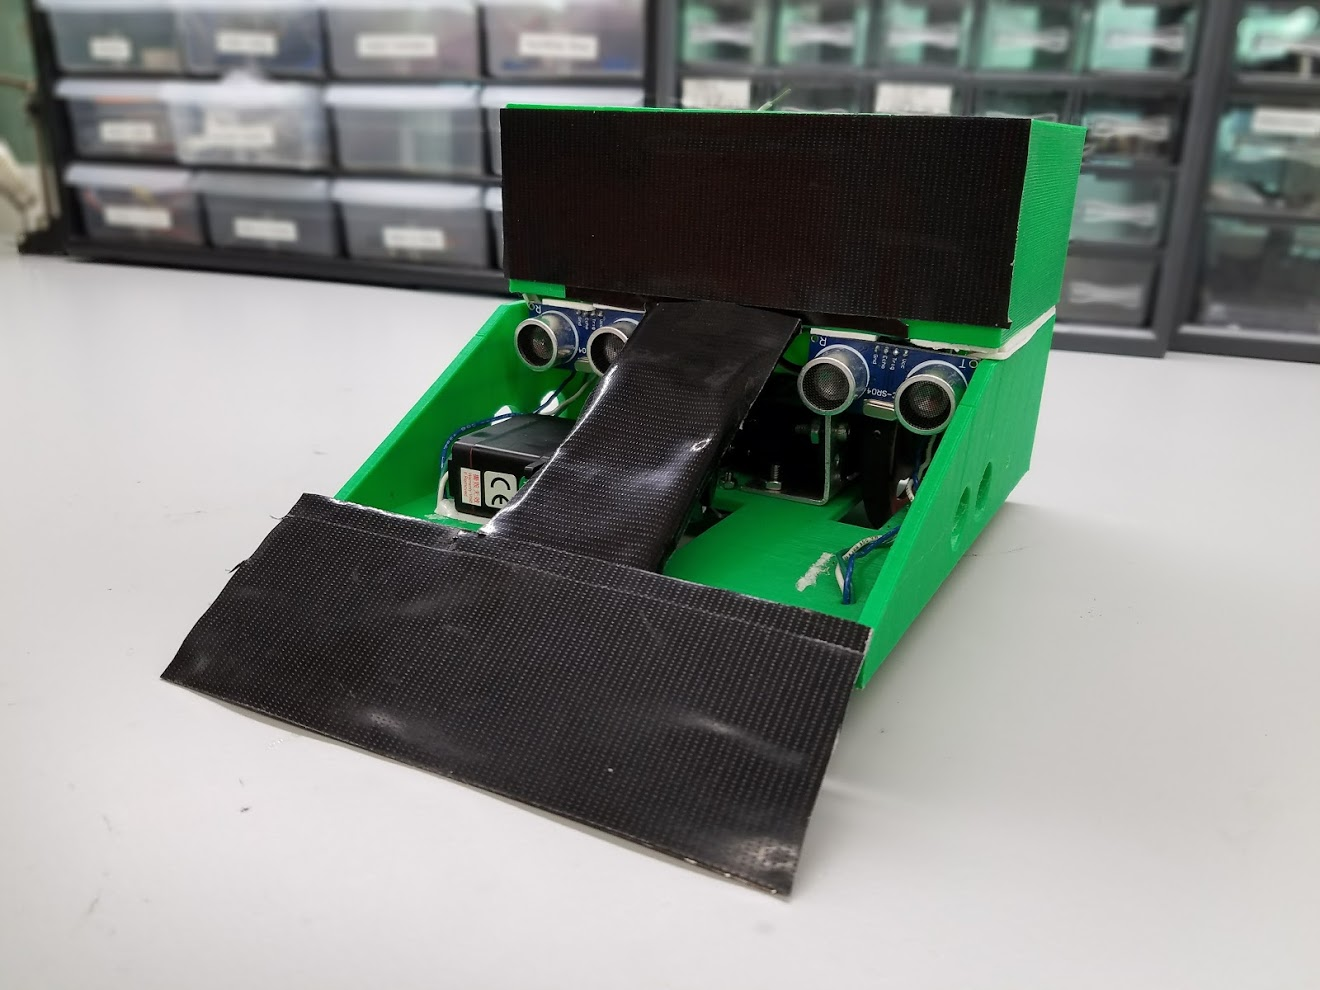
\includegraphics[scale = 0.2]{front.jpg}
		\caption{Interpreter}
		\label{fig:front}
	\end{center}
\end{figure}

We made the ``Interpreter'' for the Sumo Robot Competition, which was held as a part of the course MAE 6194. The basic functions and features of the robot are listed below.
\begin{itemize}
	\item Finds the opponent using sonar sensors
	\item Detects the line using QTI sensors
	\item If and opponent is detected, accelerates towards it
	\item If the opponent is close enough, raise the flipping shield
	\item Send every task the robot is performing through XBee
	\item Another Arduino board reads the transmitted data via an XBee, and prints to an LCD display
\end{itemize}

This report is organized as follows. First, we will discuss the details on the body structure and the sensors. Then we will be explaining how the attacking mechanism works. Next section is on details of the LCD serial monitor system which is used to continuously monitor and debug the robot. Then we will provide an overview of the overall algorithm which is used to control the robot. Finally the issues we faced and the proposed future developments. The codes are attached in the appendix.


% =================================================================================
\newpage
\section{Physical Structure}

\begin{figure}[bth]
	\begin{center}
		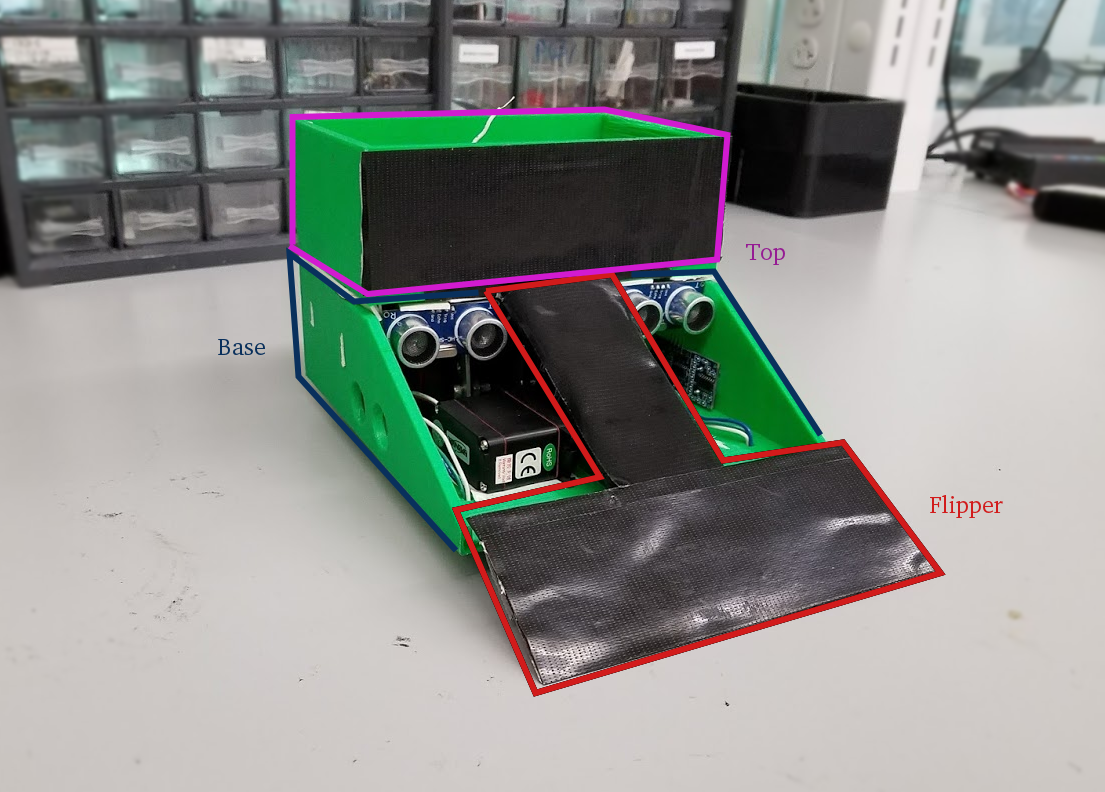
\includegraphics[scale = 0.2]{detailed_structure.png}
		\caption{Structure}
		\label{fig:detailed_structure}
	\end{center}
\end{figure}

In this section, we discuss about the body structure of the robot and the sensors. The robots structure mainly has three parts. 
\begin{enumerate}
	\item Base
	\item Top
	\item Flipper
\end{enumerate}


Base holds all the motors, back and side sonar sensors, and the QTI sensors at the bottom. On top of the Base, we have placed the Top which securely holds the Arduino board, batteries, Xbee unit, and the two front sonar sensors. Flipper is hinged to the front bottom edge of the Top and a servo motor with an arm is placed on the base, directly under the flipper, to activate the attacking mechanism.

% =================================================================================
\newpage
\section{Sensors and Components}
\subsection{Line Detection}

% =================================================================================
\newpage
\section{Attacking Mechanism}

% =================================================================================
\newpage
\section{Display System}

% =================================================================================
\newpage
\section{Algorithm}

% =================================================================================
\newpage
\section{Sumo Bot Code}

% =================================================================================
\newpage
\section{LCD System Code}

% =================================================================================
\newpage
\section{List of Components}

% =================================================================================
\newpage
\section{Future Developments}


\end{document}